\documentclass{article}
\usepackage{verbatim}
\usepackage{graphicx}

\begin{document}
\setcounter{section}{2}
\begin{center}
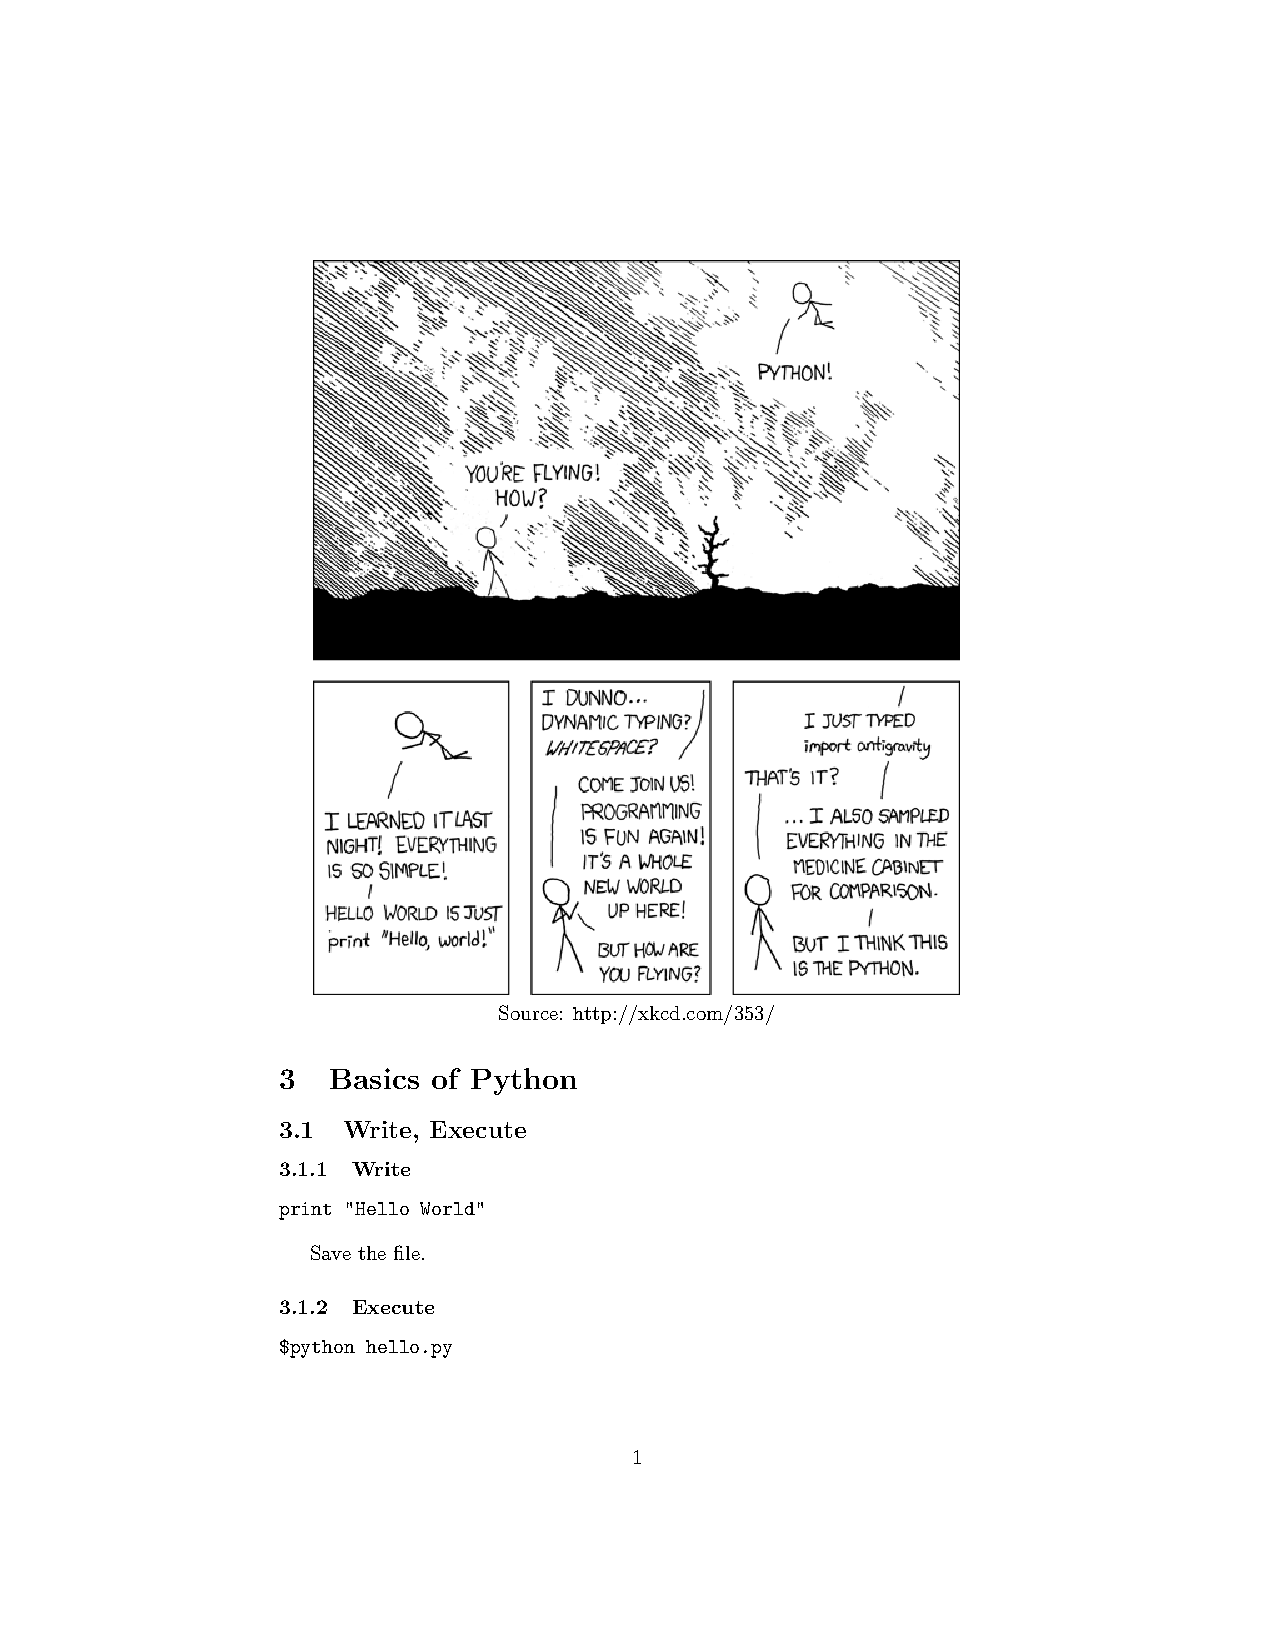
\includegraphics[scale=0.60]{python.png}
Source: {\texttt http://xkcd.com/353/}
\end{center}
\section{Basics of Python}
Python is a {\bf high-level} language. There are big advantages in
working with such languages. The most important is that they are
faster to write and easier to read. You won't have to declare the type
of the variables or allocate the memory by yourself  

In these kind of languages the compiling process is absent. You start
writing source code and then feed-it into an interpreter which is in
charge of executing thr program. The interpretation and execution
occur alternately. In the case of a {\bf low-level} language the
compiler reads and translates the source code before execution. 

Python source code is exectuted by an interpreter that you can call
from the terminal: 
\begin{verbatim}
$python
Python 2.7.3 (default, Aug  1 2012, 05:14:39) 
[GCC 4.6.3] on linux2
Type "help", "copyright", "credits" or "license" for more information. 
>>> 
\end{verbatim}

The prompt \verb">>>" indicates that the Python interpreters is ready
to receive instructions, after each instruction the interpreter
displays the result. For instance 

\begin{verbatim}
>>> 1
1
\end{verbatim}

or in the case of arithmetic operations

\begin{verbatim}
>>> 2+2
4
\end{verbatim}

You can also interact with the interpreter by writing all the lines
that you want to be interpreted into a text file with the extension
\verb".py". In that case the interpreation and execution can be called
from the terminal as follows. 

\begin{verbatim}
$ python mycode.py
\end{verbatim}

We are interested in covering the very basics of python. The recommended reference is the online text:

\begin{itemize}
\item Think Python: How to Think Like a Computer Scientist, Allen
  B. Downey.\\\verb"http://www.greenteapress.com/thinkpython/html/index.html" 
\end{itemize}

After knowing the basics a very useful repository for doing simple
things with Python is here:  


\begin{itemize}
\item Python Grimoire: \\\verb"https://taoofmac.com/media/dev/Python/Grimoire/grimoire.html"
\end{itemize}

In what follows I go through basic concepts in python with examples

\subsubsection{My first pytho program}

Save the following code in a file \verb"hello.py"
\verbatiminput{../hands_on/python/hello.py}

Then execute it as:
\begin{verbatim}
$python hello.py
\end{verbatim}

\subsection{Variables and Statements}
You don't need to declare the type of the variable before using them. 
 

\verbatiminput{../hands_on/python/variables.py}


You can also perform simple arithmetic operations


\verbatiminput{../hands_on/python/arithmetic.py}

advanced functions can should be used in the following way

\verbatiminput{../hands_on/python/math.py}


\subsection{Conditionals}
The most common way to control the flow with the program is with the
\verb"if", \verb"else", \verb"elif" and \verb"while" statements

\verbatiminput{../hands_on/python/if_while.py}


\subsection{Iteration}
\verbatiminput{../hands_on/python/print_table.py}
\subsection{Strings}

\subsection{Functions}

The definition of functions follows the generic form:

\begin{verbatim}
def function_name(inputs):
    statements
\end{verbatim}

The indentations of the statements is {\bf very important}.  This is
the way the interpreter recognizes the end and the beginning of your
function. Here is an example of two functions   


\verbatiminput{../hands_on/python/functions.py}

\subsection{Lists}
One of the most basic and useful structures in python are lists. They
can include any kind of variable.

A list can be defined as:
\begin{verbatim}
my_list = ["Apple", 3.40, 1, "Hello world"]
\end{verbatim}

the following code would print all the items in the previous list
\begin{verbatim}
print my_list[0]
print my_list[1]
print my_list[2]
print my_list[3]
\end{verbatim}

If you want to print the first item to the third

\begin{verbatim}
print my_list[0:3]
\end{verbatim}

Or if you want to iterate over each item in the list and do something
with them:

\begin{verbatim}
for item in list:
    new_item = 2 * item
    print new_item
\end{verbatim}

\subsection{Reading files}

\verbatiminput{../hands_on/python/read_file.py}

\end{document}
